
% 1986 pretrends

\begin{figure}[h]
    \centering
    \caption{College Enrollment Around 1984}%
    \subfloat[\centering By race]{{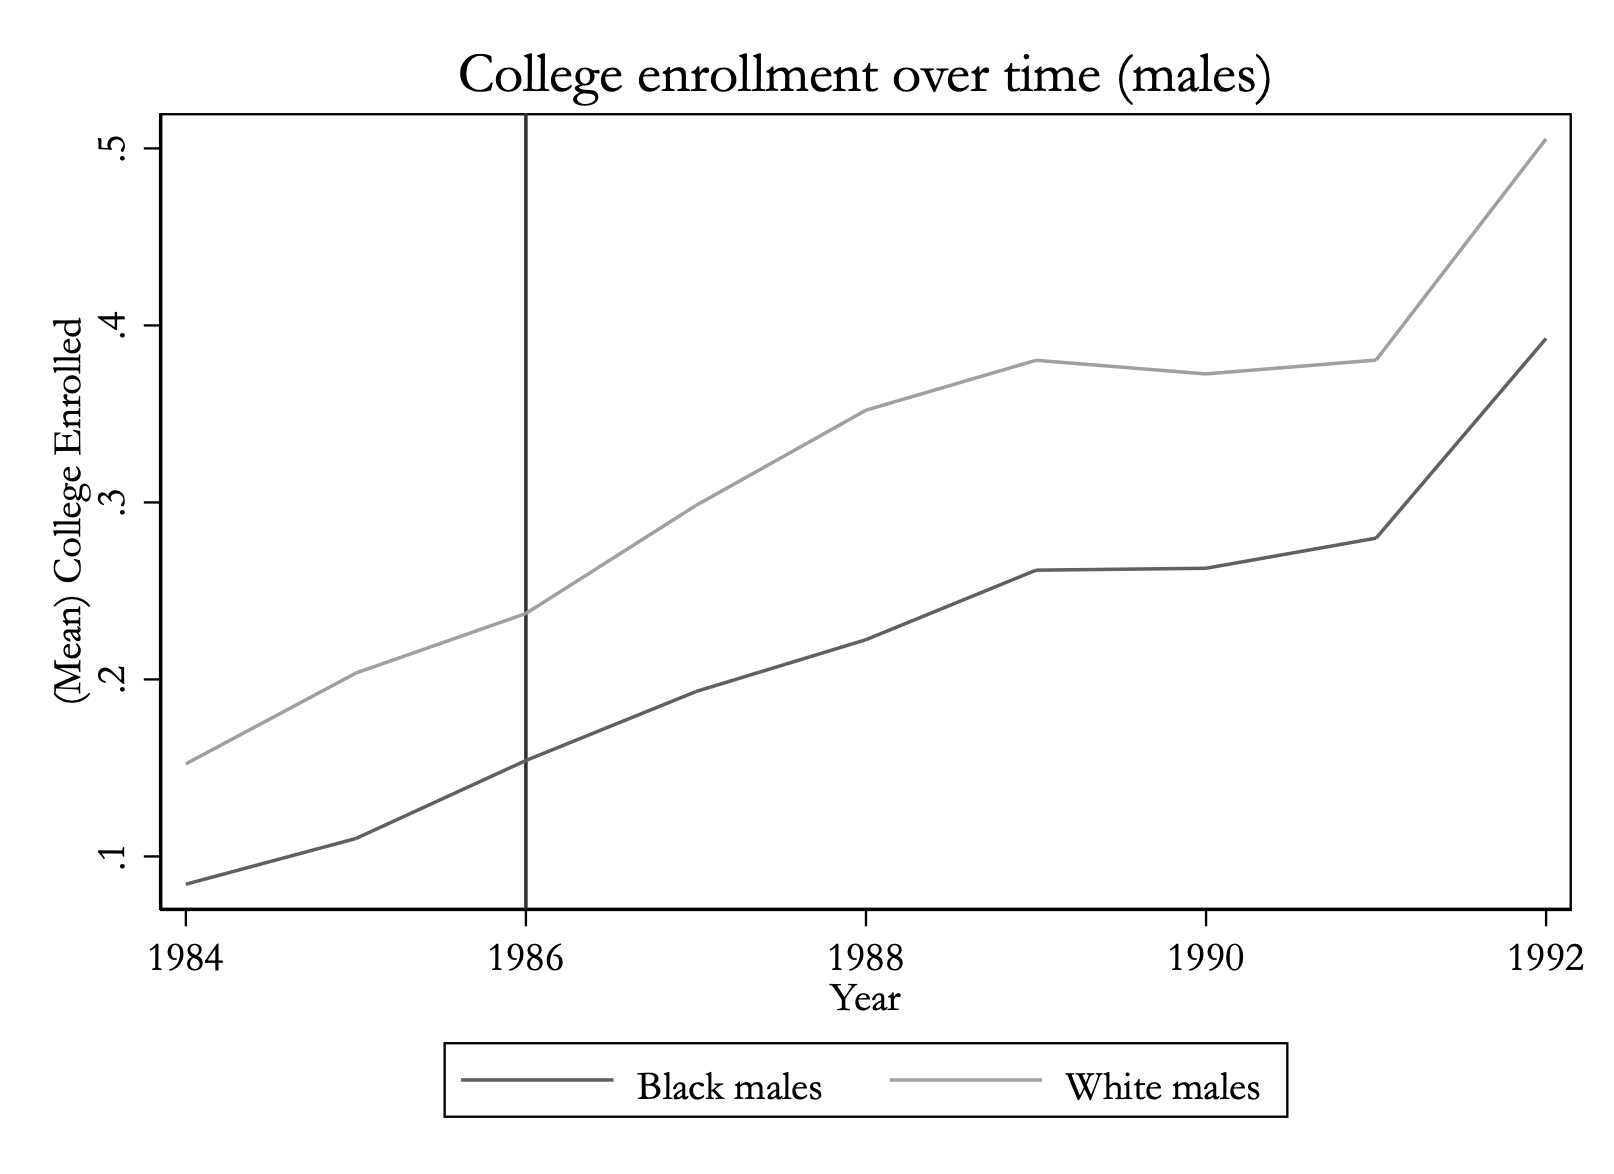
\includegraphics[width=7cm]{pretrends/1986/college_enroll_byrace_1986.png} }}%
    \qquad
    \subfloat[\centering By sex]{{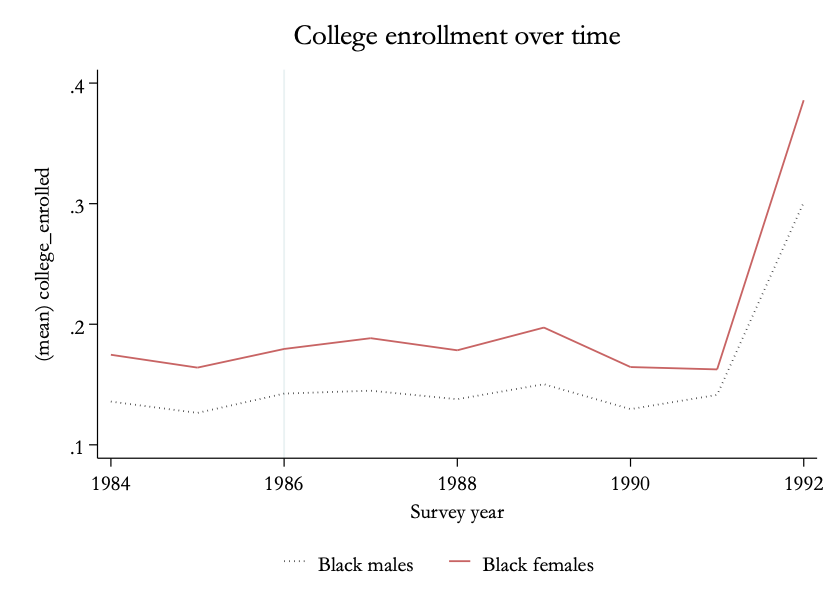
\includegraphics[width=7cm]{pretrends/1986/college_enroll_bysex_1986.png} }}%
    \label{fig:raw_college_1986}%
  \end{figure}
  
  \begin{figure}[h]
    \centering
    \caption{Family Income Around 1984}%
    \subfloat[\centering By race]{{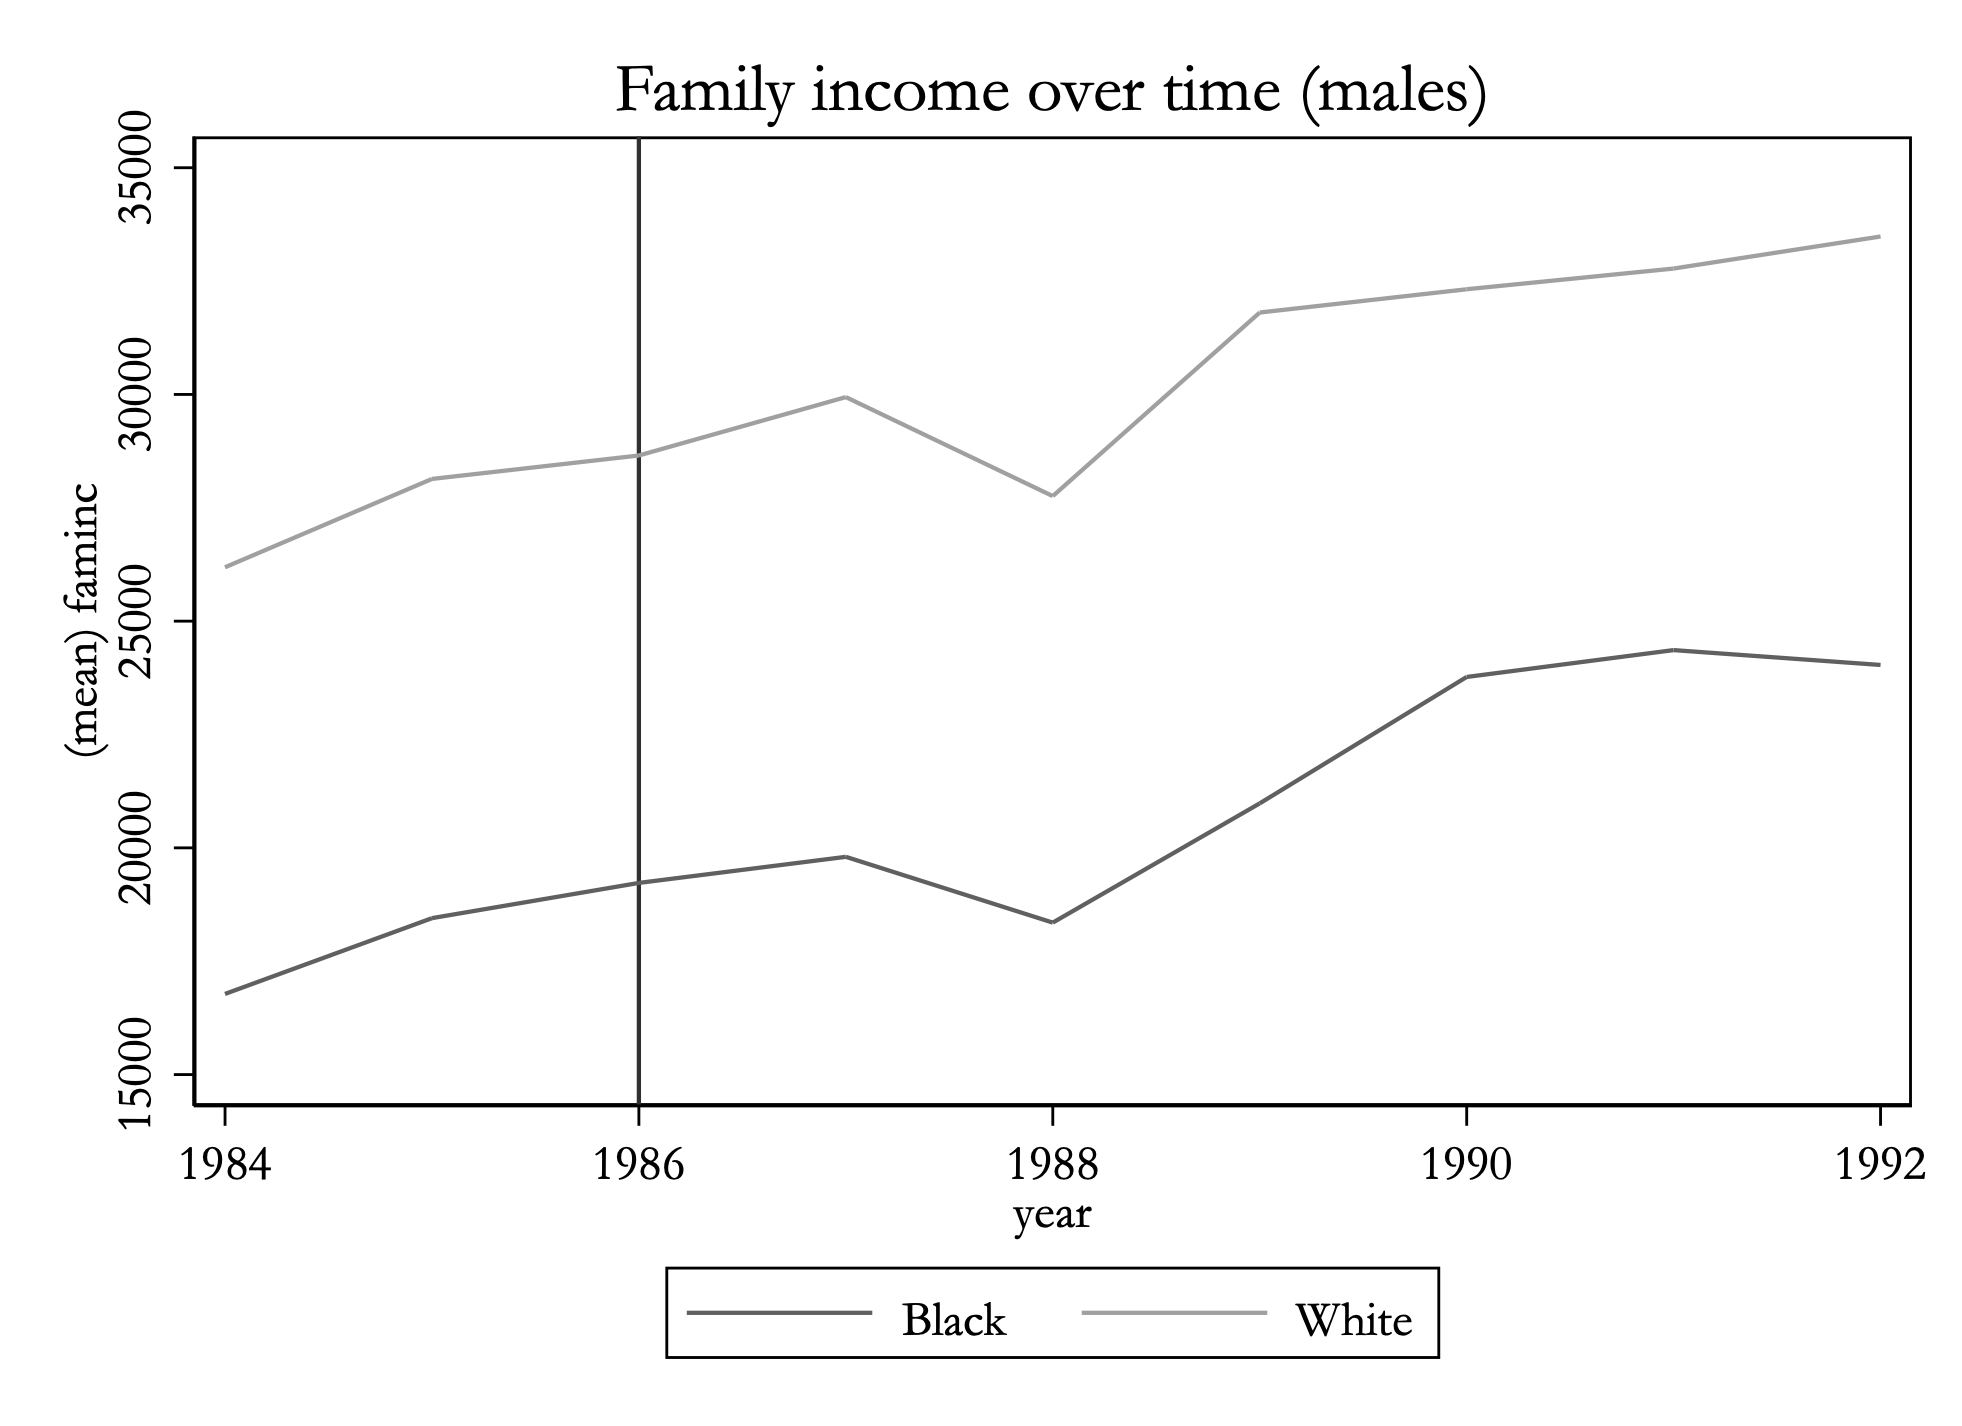
\includegraphics[width=7cm]{pretrends/1986/faminc_byrace_1986.png} }}%
    \qquad
    \subfloat[\centering By sex]{{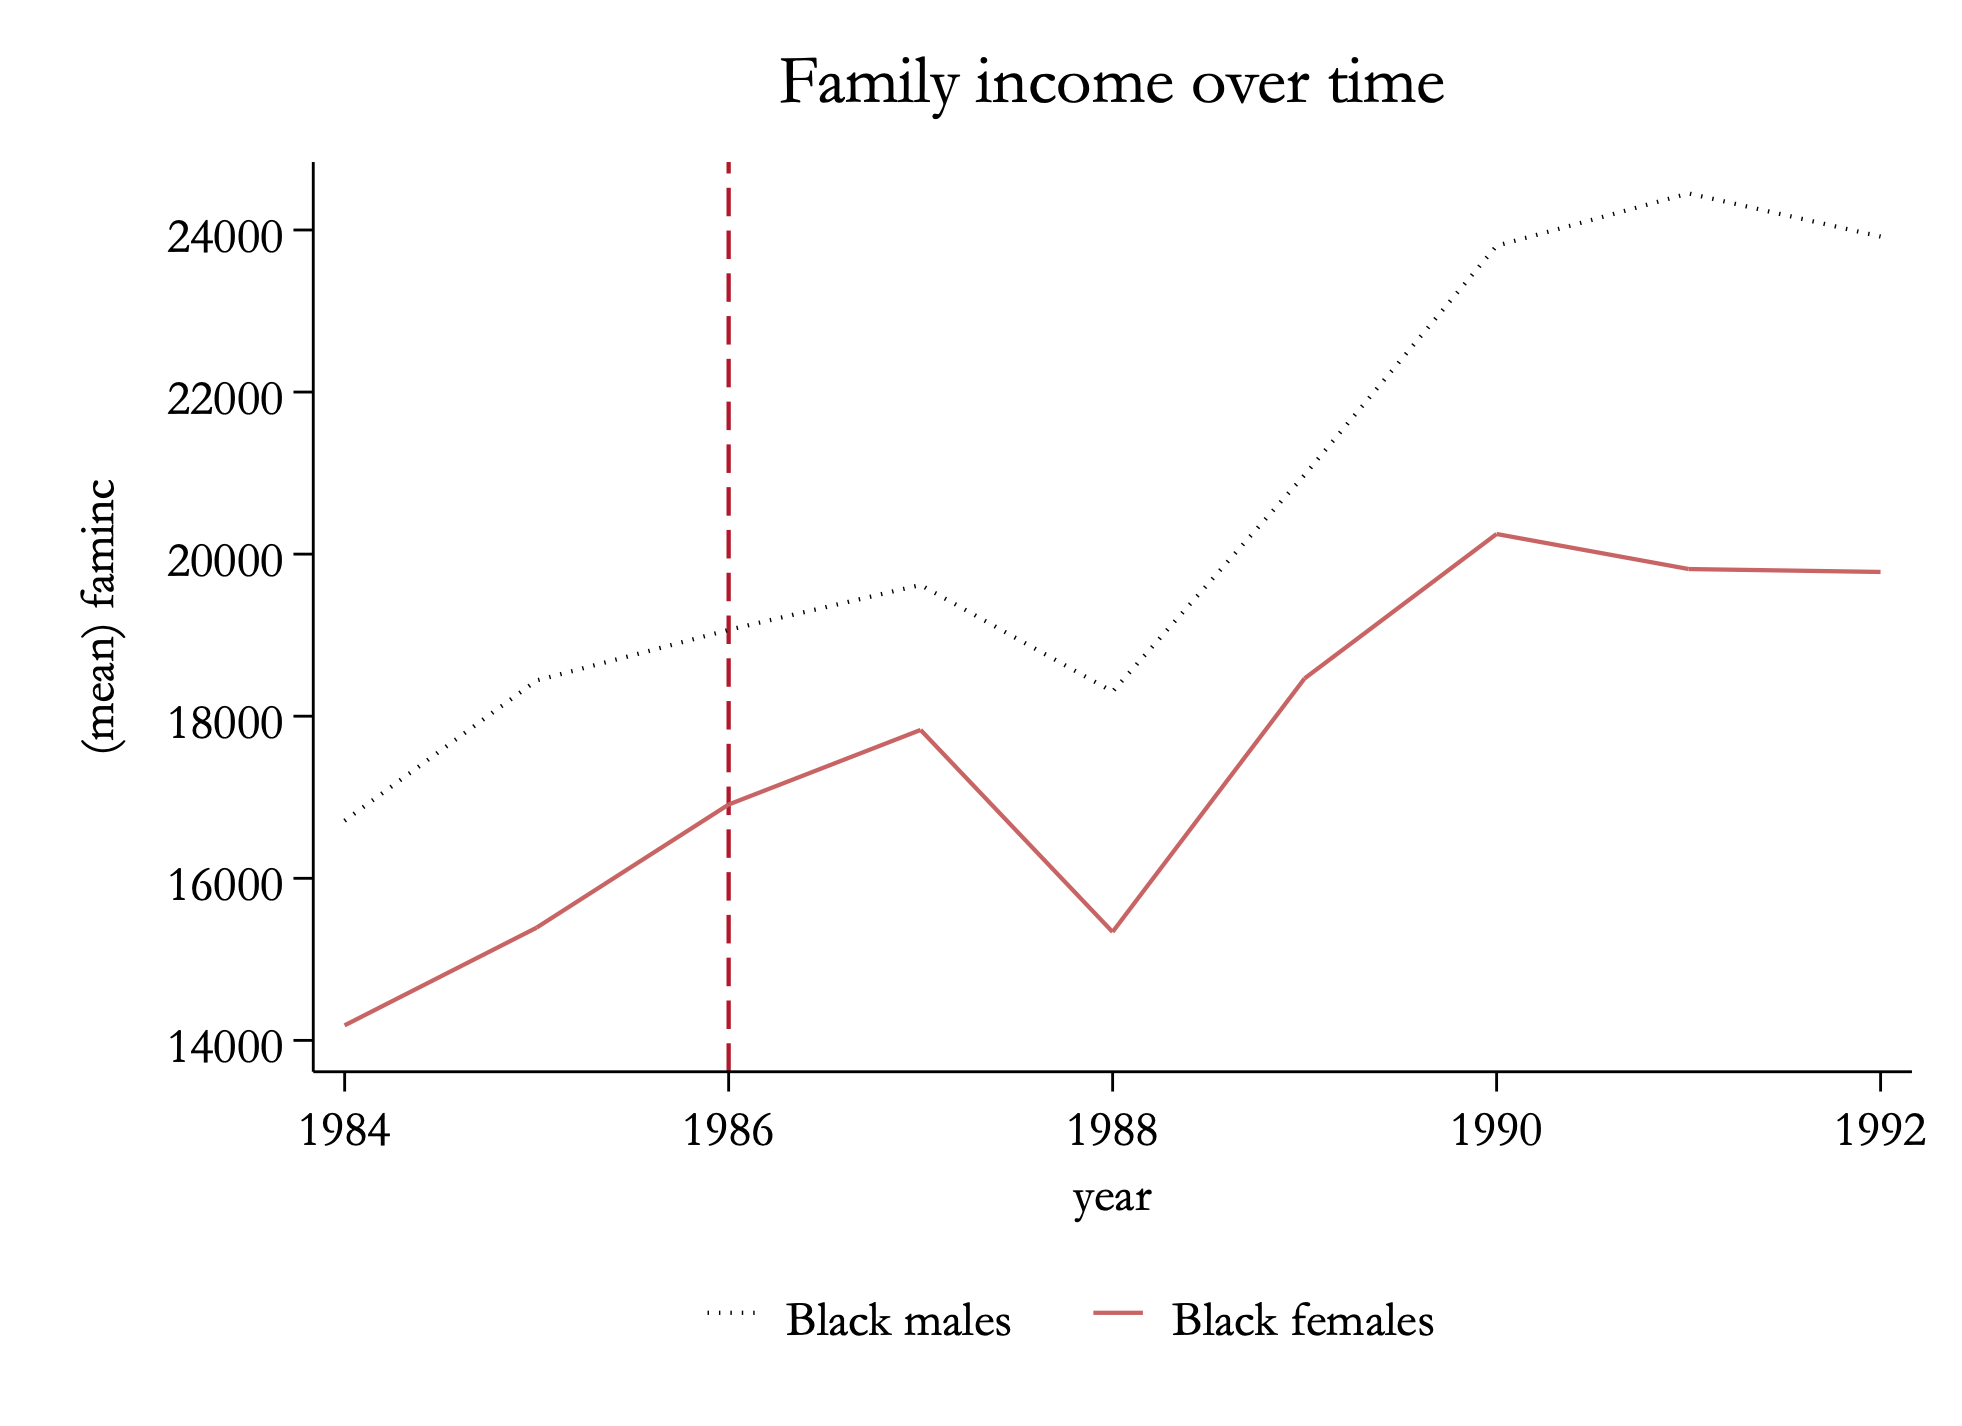
\includegraphics[width=7cm]{pretrends/1986/faminc_bysex_1986.png} }}%
    \label{fig:raw_faminc_1986}%
  \end{figure}
  
  \begin{footnotesize}
    \noindent Note: These figures report the outcomes for various subgroups plotted over time using CPS data from 1984-1992. Figure \ref{fig:raw_college_1986} reports the proportion enrolled in college, while figure \ref{fig:raw_faminc_1986} reports the average family income. A vertical line is drawn to denote the passage of the Anti-Drug Abuse Act of 1986. The universe of samples is defined as participants aged 18-24 in 1986 who were not incarcerated at the time of the survey.
  \end{footnotesize}
  
  \clearpage
  


  \clearpage

  \begin{figure}[h]
    \caption{Effect of Anti-Drug Abuse Act on Drug-related Arrest Rate of Adult Black Men, Comparing States with High and Low Black Adult Drug-Related Arrest Rates}
    \centering
    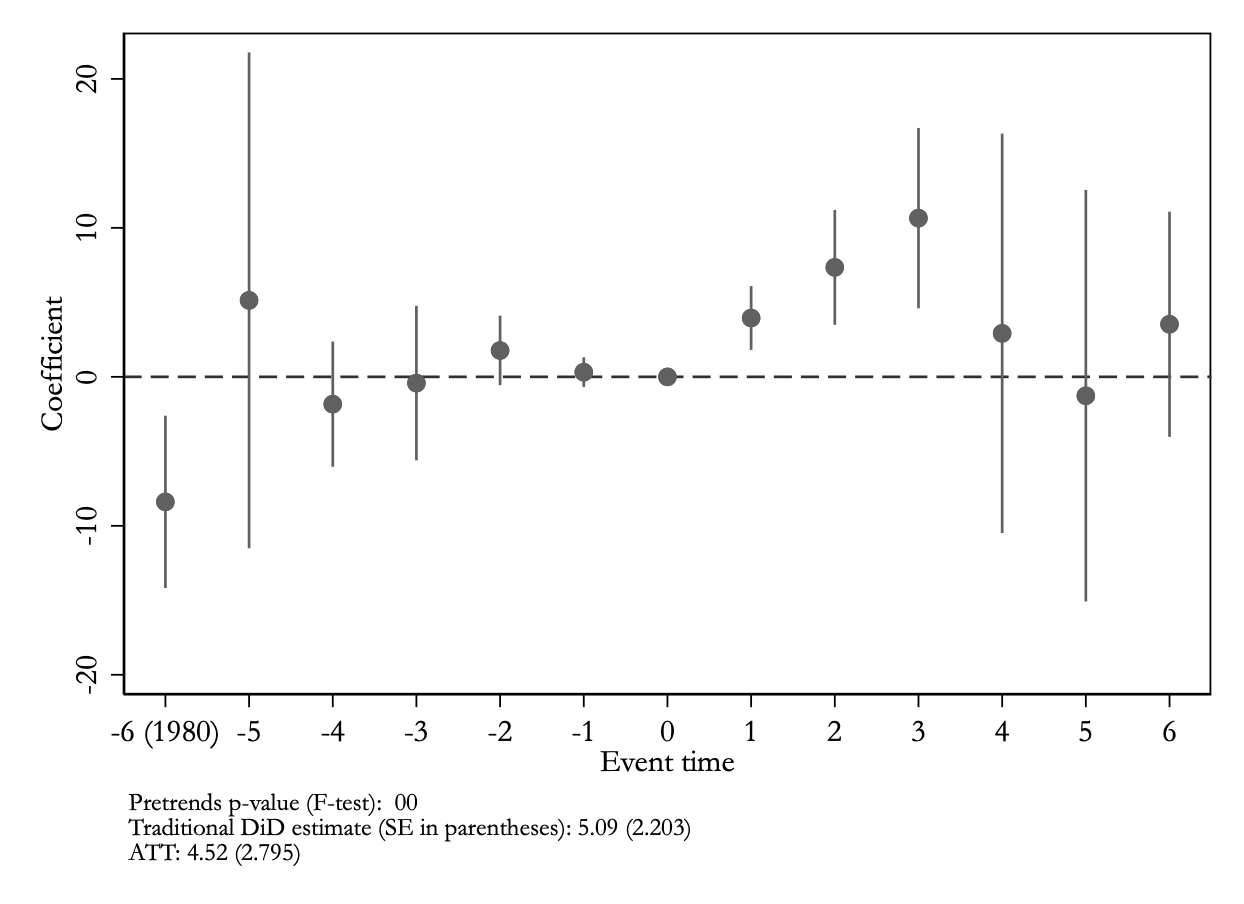
\includegraphics[width=1\textwidth]{eventstudy/high_drug_use/high_drug_eventstudy_1986_extended_years.png}
    \label{fig:a3}
  \end{figure}
  \begin{footnotesize}
    \noindent Note: This figure reports coefficients from the estimation of equation \ref{eq:state_level_es} evaluating the impact of the Anti-Drug Abuse Act of 1986 on arrest rates per 100,000 related to drug violations using CPS and UCR data from 1982-1992. Event time $0 \coloneqq 1986$. The coefficients represent the change in outcomes for high-drug arrest states relative to non-high-drug arrest states, where high black adult drug arrest states are defined to be those above the 75th percentile in 1984. The sample is defined as black males aged 18-24 in 1986 who were not incarcerated at the time of the survey. Control variables include population and unemployment rates at the state-year level. Right tail arrest rate outliers were winsorized at the 95\% level.
  \end{footnotesize}

